\subsection{شبیه‌سازی کانال رول استند در حضور کنترل‌کننده \lr{LQDG}}\label{roll_LQDG_section_simulation}
در بخش
\ref{quadchanell_roll}
شبیه‌سازی کانال رول استند چهارپره انجام شد. در این بخش به بررسی عملکرد چهارپره در حضور کنترل‌کننده \lr{LQDG} پرداخته می‌شود. کنترل‌کننده \lr{LQDG} در بخش
\ref{LQDG}
بررسی شده است.
 در شبیه‌سازی برای بهینه‌سازی ضرایب وزنی \lr{LQDG} از روش
\lr{TCACS} \cite{Karimi2010}
استفاده شده است.
\begin{figure}[H]
	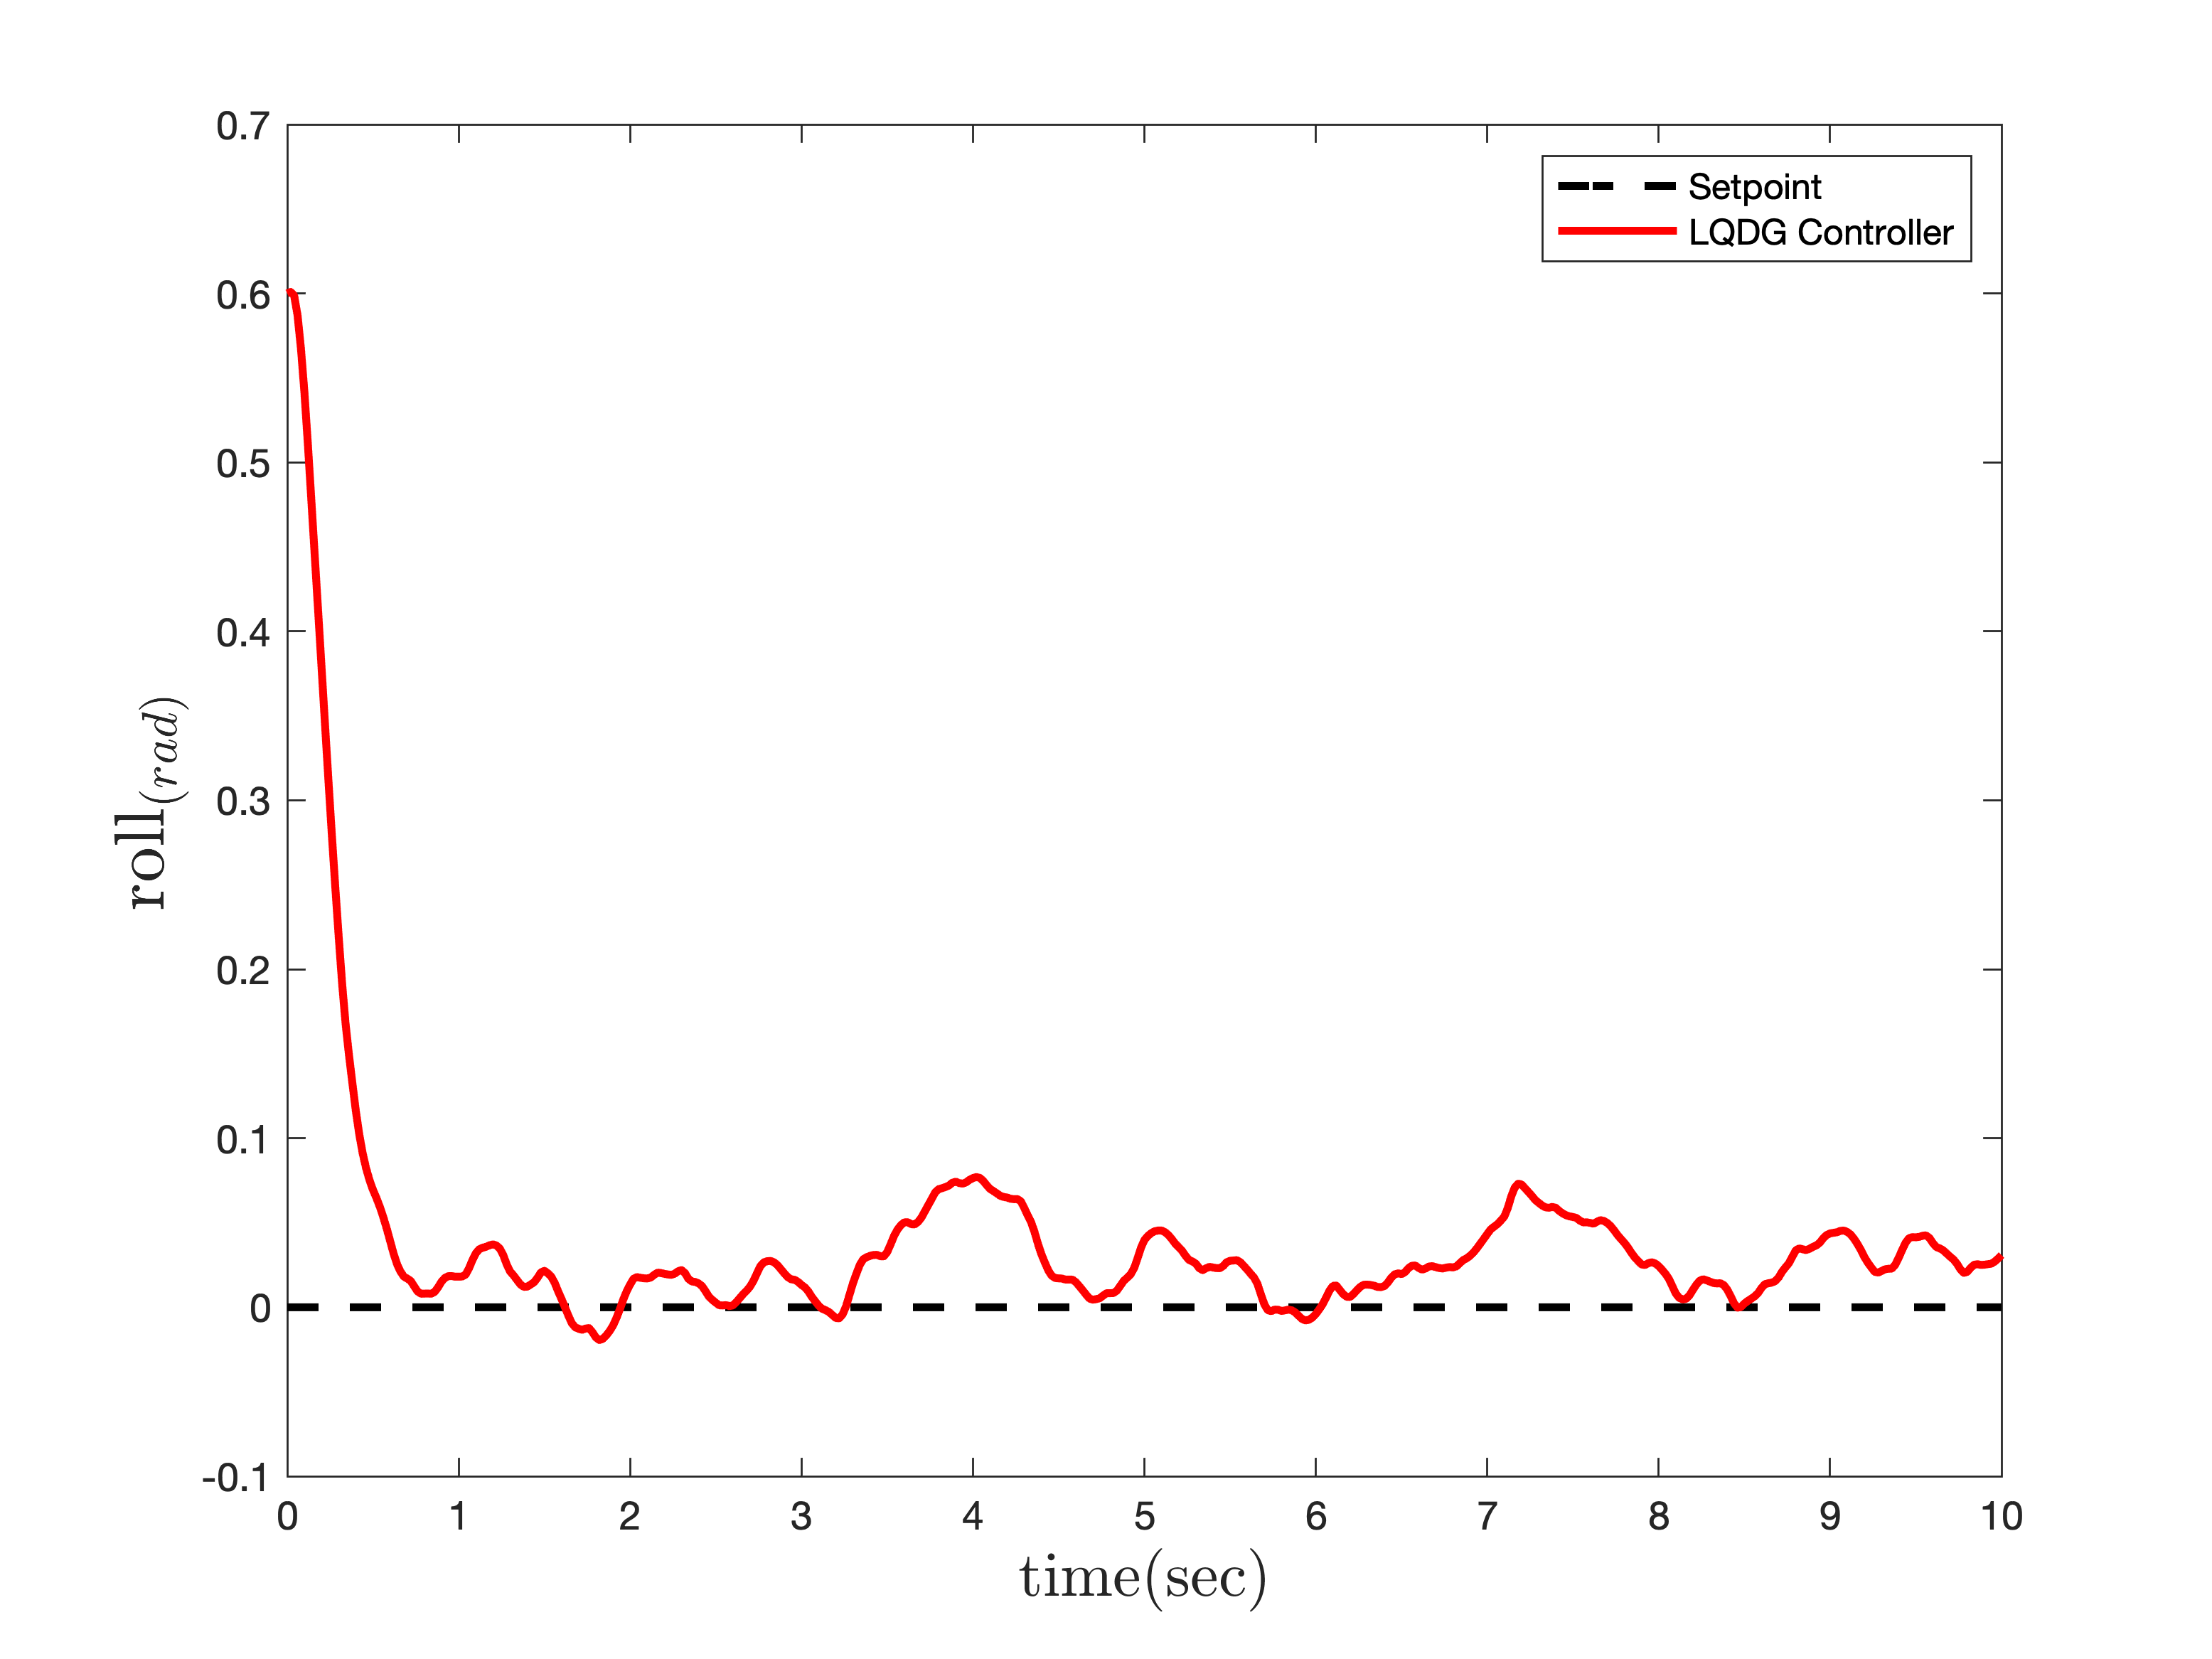
\includegraphics[width=12cm]{../Figures/MIL/LQDG/Roll/lqdg_roll.png}
	\centering
	\caption{عملكرد \lr{LQDG} در کنترل زاويه رول (تعقیب ورودی صفر)}
	\label{lqdg_roll_fig_simulation}
\end{figure}
بر اساس خروجی شبیه‌سازی (شکل
\ref{lqdg_roll_fig_simulation})
،کانال رول در حضور کنترل‌کننده \lr{LQDG} در کمتر از پنج ثانیه به تعادل می‌رسد اما دارای خطای ماندگار است ولی خطای مانگار آن نسبت به کنترل‌کننده بخش
\ref{roll_lqr_section_simulation}
کمتر است. به دلیل خطای ماندگار، در بخش
%LQIDG
انتگرال‌گیر به کنترل‌کننده اضافه می‌شود تا خطای مانگار استند را کم کند.
